At this stage in the analysis, we have no more simple cuts which can improve the signal-to-background ratio in the dataset, but we know there must still be background remaining, as is indicated by the excess events with small kaon rest-frame lifetimes seen in \Cref{fig:rfl-pre-splot}. In this figure, we see that one of the intrinsic properties of a $K_S^0$, its well-known lifetime, is not distinct in the data. Rather, we seem to have at least two exponential slopes in the rest-frame lifetime distribution of each kaon, one which is close to what we see in signal Monte Carlo, and another which is similar to the $4\pi$ background Monte Carlo. We must now turn to more elaborate methods of separating the signal from this potential background influence. The primary method we will use to do this is sPlot~\cite{Pivk2005}\footnote{This is stylized as ${}_s\mathcal{P}lot$ in the original paper, but I find this tedious to type and to read.}, a weighting scheme which corrects the na\"ive probabilistic weights one might first think to construct (dubbed ``inPlot''). We begin by giving a basic explanation of inPlot before describing the sPlot correction.

\begin{figure}
  \begin{center}
    \begin{subfigure}{.8\columnwidth}
      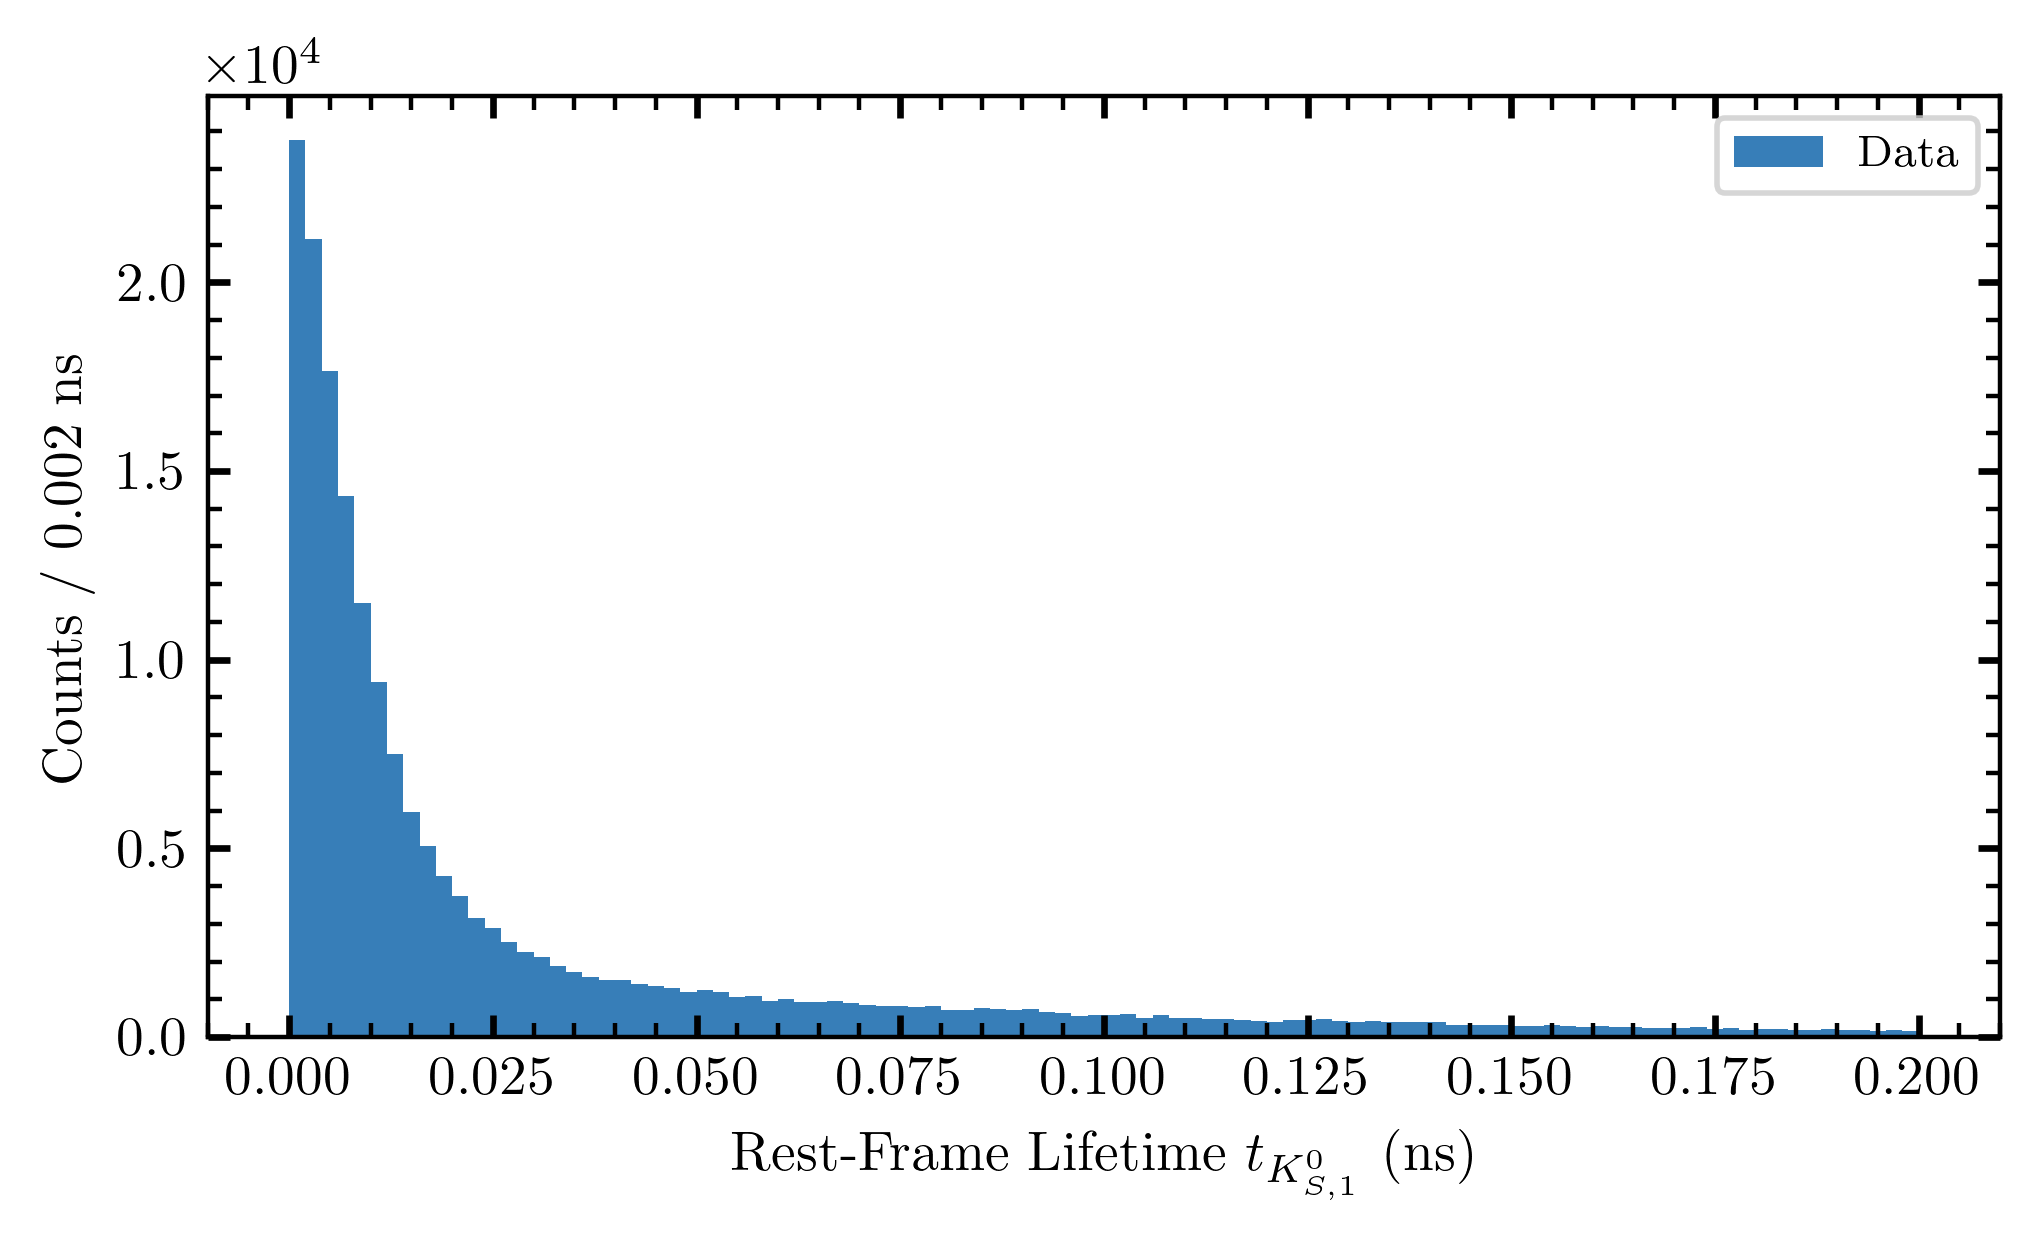
\includegraphics[width=\linewidth]{figures/rfl_data_chisqdof_3.4.png}
      \caption{Data}
      \label{fig:rfl-data}
    \end{subfigure}
    \begin{subfigure}{.45\columnwidth}
      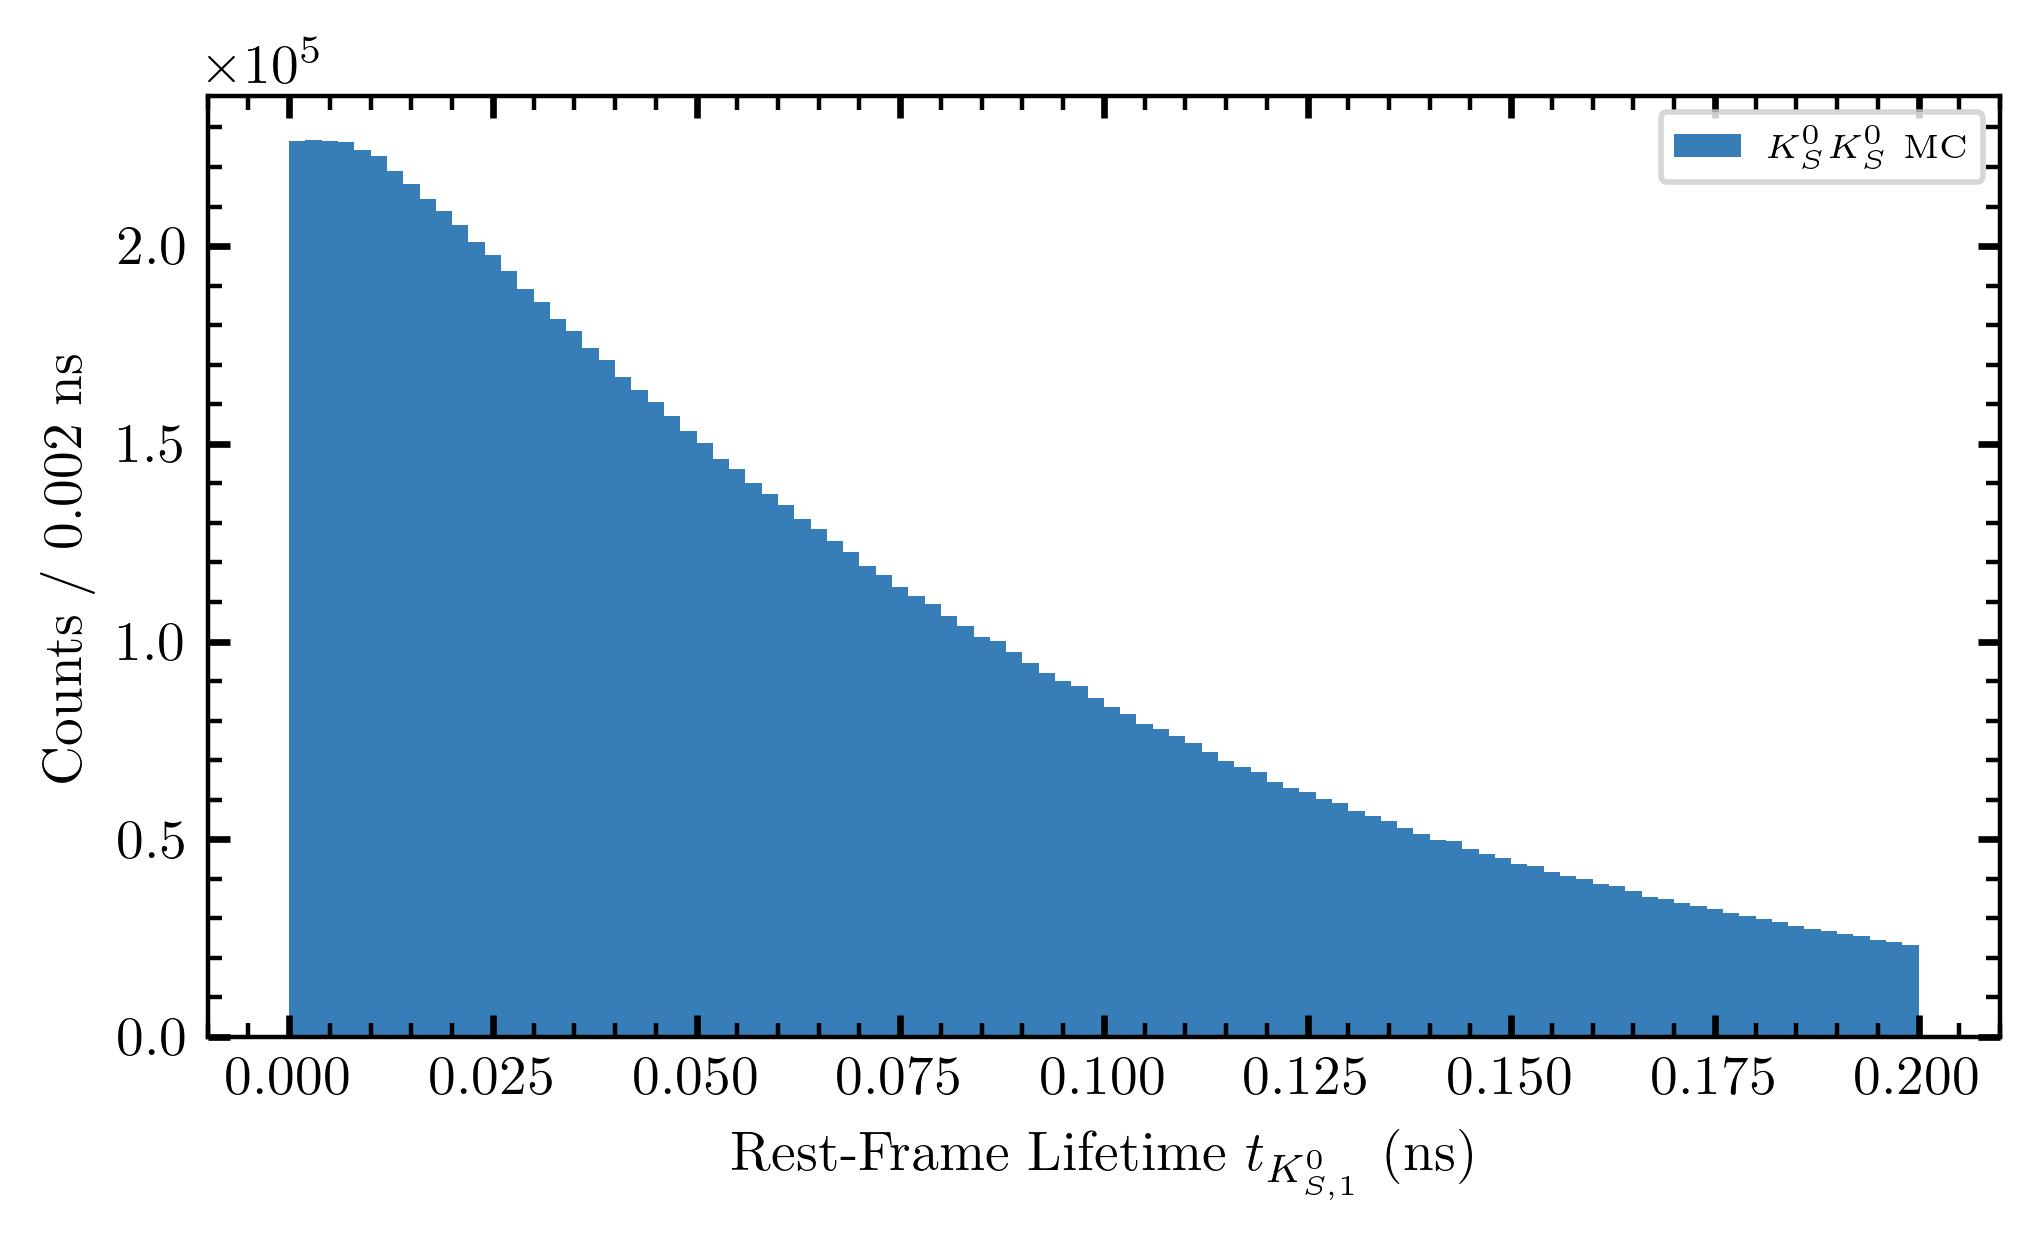
\includegraphics[width=\linewidth]{figures/rfl_accmc_chisqdof_3.4.png}
      \caption{Signal Monte Carlo}
      \label{fig:rfl-accmc}
    \end{subfigure}
    \begin{subfigure}{.45\columnwidth}
      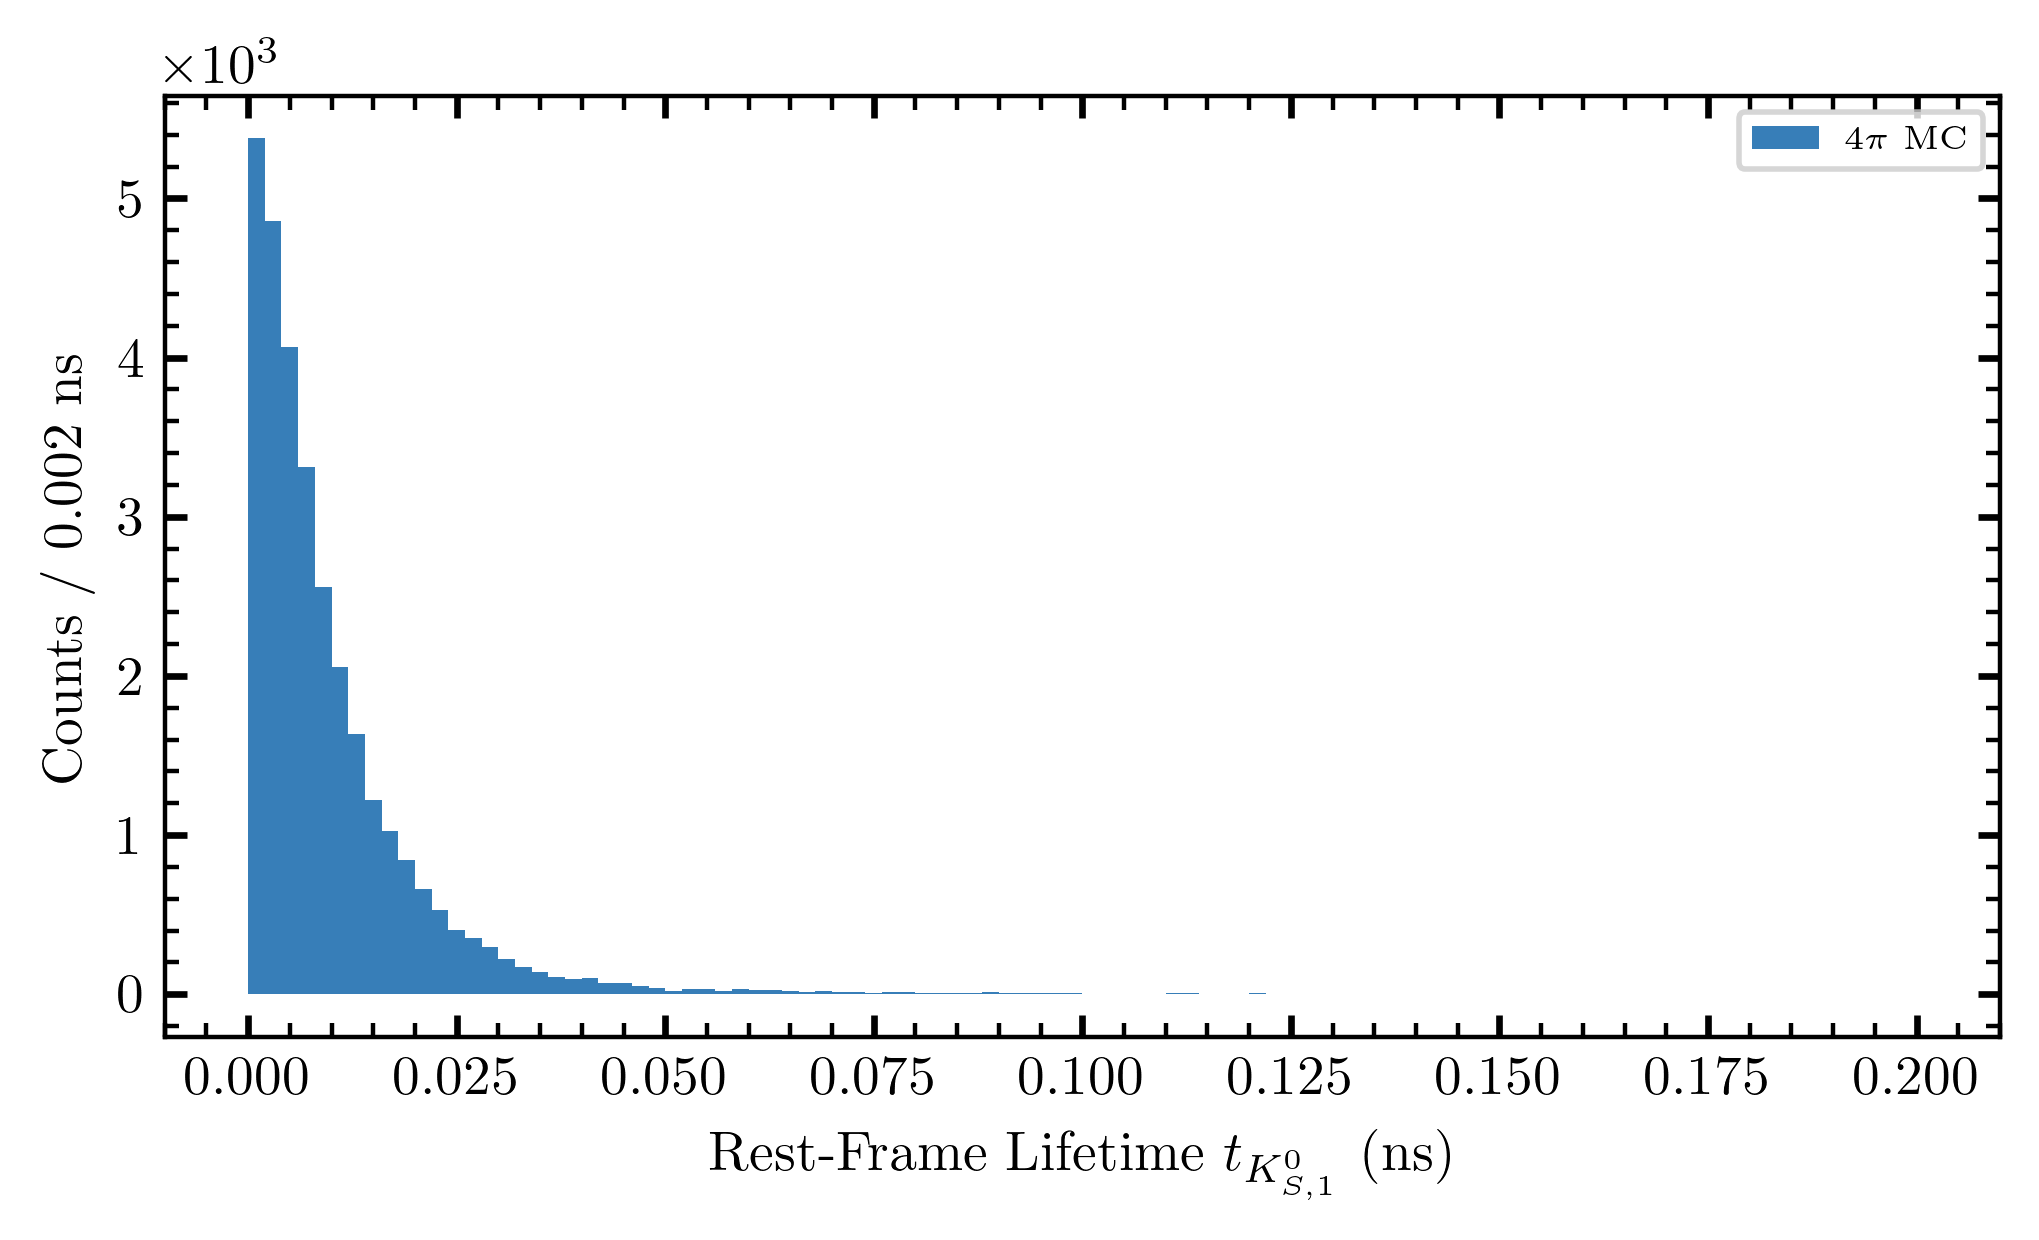
\includegraphics[width=\linewidth]{figures/rfl_bkgmc_chisqdof_3.4.png}
      \caption{$4\pi$ Background Monte Carlo}
      \label{fig:rfl-bkgmc}
    \end{subfigure}
  \end{center}
  \caption{The rest-frame lifetime of kaons in (a) data, (b) signal Monte Carlo, and (c) background Monte Carlo. The data distribution clearly contains two exponential slopes: a peak which resembles the $4\pi$ Monte Carlo distribution, and a tail of true $K_S^0$s which resembles the signal Monte Carlo.}\label{fig:rfl-pre-splot}
\end{figure}

For all of the statistical weighting methods which will be mentioned here, we need some model for the signal and background probability distribution functions (PDFs) for some ``discriminating'' variable. This variable is called ``discriminating'' because it the variable for which we know the shape of these distributions beforehand. The usual example is a ``bump-on-a-background'', in which the discriminating variable may be a mass distribution ($m$) where signal events show up as a peaking structure while background events are more uniformly distributed. In such situations, it is common to use the extremes of the mass distribution (sidebands) as estimates of the background everywhere, weighting these events negatively while the events in the peak are weighted positively (a sideband subtraction). Rather than specifying peak and sideband regions, we can fit the mass distribution to some mixture of a signal (peak) PDF $f_S(m)$ and a background (flat) PDF $f_B(m)$. From such a fit, we obtain estimated number of signal ($N_S$) and background ($N_B$) events in our dataset (and possibly some shape parameters for the signal and background PDFs). We could then assign weights to each event as in \Cref{eq:inplot-weights-mass},

\begin{equation}
  w(m) = \frac{N_S f_S(m)}{N_S f_S(m) + N_B f_B(m)},
  \label{eq:inplot-weights-mass}
\end{equation}

We might want to look at the ``signal'' inPlots for the decay angles $\theta$ and $\varphi$ (control variables) in the helicity system after calculating the inPlot weights from a fit to the mass distribution (discriminating variable). However, as shown by Pivk and Le Diberder~\cite{Pivk2005}, we can only use inPlot in cases where the control variables are statistically dependent on the discriminating variable\footnote{In practice, more than one discriminating variable can be used.}, $y$. In other words, our example would only be valid if $\theta = \theta(m)$ and $\phi = \phi(m)$. For the time being, let us assume that this is not the case, and that we wish to use the distribution of some variable which is statistically independent from the variables we are plotting and analyzing\footnote{Total statistical (in)dependence is a very strict requirement, but we will later see that small modifications to the sPlot method can permit amounts of dependence between the two extremes.}. A correction term can be applied to give us the sPlot version of \Cref{eq:inplot-weights-mass},

\begin{equation}
  w(y) = \tilde{w}(y)\frac{V_{SS}f_S(y) + V_{SB}f_B(y)}{N_S f_S(y) + N_B f_B(y)},\quad \text{where } V^{-1}_{ij} = \sum_{y} \frac{\tilde{w}(y)f_i(y)f_j(y)}{\left(N_S f_S(y) + N_B f_B(y)\right)^2},
  \label{eq:splot-weights}
\end{equation}
where $y$ represents any set of discriminating variables (not necessarily a mass), and $\tilde{w}(y)$ is any pre-existing weight associated with the event (weights from accidental subtraction, for instance). The $V^{-1}$ matrix can also be understood as the covariance matrix between the free parameters $N_S$ and $N_B$ in the fit of the signal-background mixture, $V^{-1}_{ij} = -N\pdv[2]{\ln\mathcal{L}}{N_i}{N_j}$, although there is reason to believe that direct calculation by inverting the Hessian matrix from the fit will lead to less accurate results than the manual calculation method given in \Cref{eq:splot-weights}~\cite{Dembinski2022}.

Now that we have a method of assigning weights, we must pick the discriminating variables. As mentioned, these weighting methods work well on the classic ``bump-on-a-background'' distributions because it is easy to identify the signal and background PDFs, but because the mass of the kaons is constrained in the kinematic fit, the fitted mass of each kaon is just a $\delta$-function and combination of measured masses for each $\pi^+\pi^-$ pair will yield a Normal distribution with little to no apparent background (by construction), so we must be a bit more clever in selecting discriminating variables. By examining the \texttt{bggen} analysis done in \Cref{sec:data-selection}, we can see that most likely sources of background arise when the intermediate kaons are absent from the reaction: $\gamma p \to 4\pi p$. This reaction has the $K_SK_S$ final state, so pairs of pions which reconstruct close enough to kaons will be almost indistinguishable in the data. However, they differ in one key way, namely that the $K_S$ intermediate contains a strange quark while the $\pi^+\pi^-$ decay state does not, so such a decay must occur via the weak interaction, which is notably slower than the strong interaction which would produce pion pairs with no intermediate kaon. In other words, while the signal's rest-frame lifetime distribution should have an exponential slope near the $K_S$ lifetime, the background would theoretically have nearly zero rest-frame lifetime for every event, or a much smaller exponential slope in practice\footnote{An exponential distribution is just what fits the rest-frame lifetime distribution in the $4\pi$ Monte Carlo best and has no other physical implication.}.

Therefore, we will begin by generating both a signal and background dataset in Monte Carlo. We then interpret both datasets as if they were our desired channel by running them through the GlueX reconstruction and reaction filter, as well as all of our selections up to this point. The signal Monte Carlo distribution in \Cref{fig:rfl-accmc} mostly follows an exponential distribution, but it flattens out near zero. Rather than use an exponential model, we will use the shape of this distribution itself, as it includes acceptance effects from the detector. The background distribution is roughly exponential, so we will fit the background Monte Carlo to an exponential distribution,

\begin{equation}
  f(t; \lambda) = \lambda \exp{-\lambda t},
  \label{eq:splot-exponential}
\end{equation}
where $\lambda \equiv 1/\tau$, the lifetime of the (hypothesized) kaon in question. To account for the fact that there could be backgrounds other than the one we simulated, we will allow the slope of this background distribution to vary, although we will start the fit at a value obtained from the Monte Carlo simulation. Since we have two independently decaying kaons, we should really form a joint distribution for both, where we will assume each kaon has the same average lifetime:
\begin{equation}
  f(t_1, t_2; \lambda) = \lambda^2 \exp{-\lambda t_1}\exp{-\lambda t_2}
  \label{eq:splot-exponential_joint}
\end{equation}

As mentioned previously, rather than model the signal distribution analytically, we will instead use the distribution from the Monte Carlo itself as the model by binning the simulated data (a bin width of $\SI{1}{\pico\second}$ seems to give a distribution that is decently smooth in practice). In the following discussions, we will use this binned distribution as the model for the signal component and the exponential distribution in \Cref{eq:splot-exponential_joint} for the background component. Because of this, the signal distribution does not have a slope parameter, so we construct a mixture equation which looks like,

\begin{equation}
  g(t_1, t_2; z, \lambda_B) \equiv z \tilde{f}(t_1, t_2) + (1-z) f(t_1, t_2; \lambda_B),
  \label{eq:splot-mixture}
\end{equation}
where $\tilde{f}$ represents the binned distribution, and $z$ is the signal fraction ($N_S = z\cdot N$ and $N_B = (1-z)\cdot N$ where $N_S$ is the number of signal events, $N_B$ is the number of background events, and $N = N_S + N_B$ is the total number of events), and the equation for the likelihood is,

\begin{equation}
  -2\ln\mathcal{L}(z,  \lambda_B) = -2\sum_i^N \tilde{w}_i \ln g(t_{1,i}, t_{2,i}; z, \lambda_B)
  \label{eq:splot-nll}
\end{equation}

\subsection{Non-Factorizing sPlot}\label{sec:non-factorizing-splot}

Over the course of the previous discussion, it was assumed that the discriminating variables, $t_1$ and $t_2$, were statistically independent from the control variables we wish to use in later analyses. The set of control variables must include all variables we use as inputs to the partial-wave analysis in \Cref{ch:partial-wave-analysis}, including the invariant mass $m$ of the $K_S^0K_S^0$ system and the helicity angles $\theta$ and $\varphi$ of the decay. We should now confirm that the rest-frame lifetimes are statistically independent from these control variables (in other words, show that they are statistically independent). To test for statistical independence between $t_{1,2}$ and a given control variable, we first split our dataset into $M$ evenly-spaced quantiles in that control variable, which ensures each bin gets roughly the same number of events. Next, we calculate the likelihood of a null hypothesis which assumes the variables are statistically independent by fitting all datasets simultaneously with a shared $\lambda_B$ parameter. We then calculate the likelihood of an alternative hypothesis, which assumes statistical dependence, by finding the joint likelihood of independent fits of $\lambda_B$ over each quantile. The result of these fits can be formulated as a likelihood ratio,

\begin{equation}
  \Lambda = -2\ln\frac{\sup \mathcal{L}_{H_0}}{\sup \mathcal{L}_{H_1}} = -2\ln\frac{\sup \prod_i^M \mathcal{L}_i(z_i, \lambda_B)}{\sup \prod_i^M \mathcal{L}_i(z_i, \lambda_{B,i})},
  \label{eq:independence-test}
\end{equation}
where $\mathcal{L}_{H_0}$ and $\mathcal{L}_{H_1}$ are the likelihoods of the null and alternative hypotheses respectively, the supremum indicates we are maximizing these likelihoods (in a maximum likelihood fit), the product $\prod_i^M$ iterates over each quantile of data in the given control variable, and $\mathcal{L}_i$ is the likelihood evaluated over data in the $i$th quantile. $\Lambda$ is $\chi^2$ distributed with $M - 1$ degrees of freedom (the difference between $M + 1$ free parameters in the null hypothesis, a signal fraction $z_i$ for each quantile plus the exponential background slope shared across all quantiles, and $2M$ in the alternative hypothesis, a signal fraction and one exponential slope for each quantile). The factor of $2$ is required because $\ln\mathcal{L}(\theta_1,...,\theta_i) \sim -\frac{1}{2}\chi^2_i$ asymptotically with sample size, according to Wilks' theorem. We can obtain a $p$-value representing the likelihood of the null hypothesis being true by evaluating the $p$-value:

\begin{equation}
  p = 1 - F_{\chi^2_{M-1}}(\Lambda),
  \label{eq:significance-test}
\end{equation}
where $F_{\chi^2_{M-1}}(\Lambda)$ is the cumulative distribution function of a $\chi^2$ distribution with $M-1$ degrees of freedom. Following this procedure for the invariant mass of $K_S^0K_S^0$\footnote{No significant statistical dependence was found for the helicity angles.}, we obtain $p$-values of $<2.23\times10^{-308}$ with two, three, or four quantiles. The calculated $p$-values imply that we should reject the null hypothesis and accept that the discriminating (rest-frame lifetime) and control (invariant mass of $K_S^0K_S^0$) variables are not statistically independent. This means we cannot use a traditional sPlot to weight our data.

The results of these tests over the data consistently return $p$-values close to zero (below machine precision). While this may seem surprising, the results are visualized for four quantiles in \Cref{fig:factorization}, and we can see that there is a strong statistcal dependence between the control and discriminating variables which lead to this low $p$-value. Again, the significantly small $p$-values justify the use of non-factorizing sPlot across the background component, meaning that we need at least two background components in the final sPlot weighting\footnote{We found that a similar analysis an exponential signal distribution also indicates a significant amount of non-factorization, but the difference in the slopes of each component are too small to give significantly different fits to the true data. Additionally, we could choose to use the Monte Carlo distribution for the background as well, but that would assume that we have correctly modeled the entire background, while we really only modeled what we believe was the most prominent component.}.

The process for obtaining the correct weights is straightforward, we simply allow for more than one signal and background component in the fit and sum over all signal components when we calculate the final weight values~\cite{Dembinski2022}. Since the weights corresponding to each signal component in the sPlot can be added to each other to obtain a joint weight~\cite{Pivk2005}, \Cref{eq:splot-weights} can be extended to allow multiple signal and background components:

\begin{equation}
  w(y) = \frac{\sum_{j} V_{Sj}f_j(y)}{\sum_{k}N_kf_k(y)},\quad \text{where } V_{ij}^{-1} = \sum_{y} \frac{f_i(y)f_j(y)}{\left(\sum_{k} N_kf_k(y)\right)^2}
  \label{eq:splot-weights-factorizing}
\end{equation}

and $S$ is the index of the signal component.


\begin{figure}
  \begin{center}
    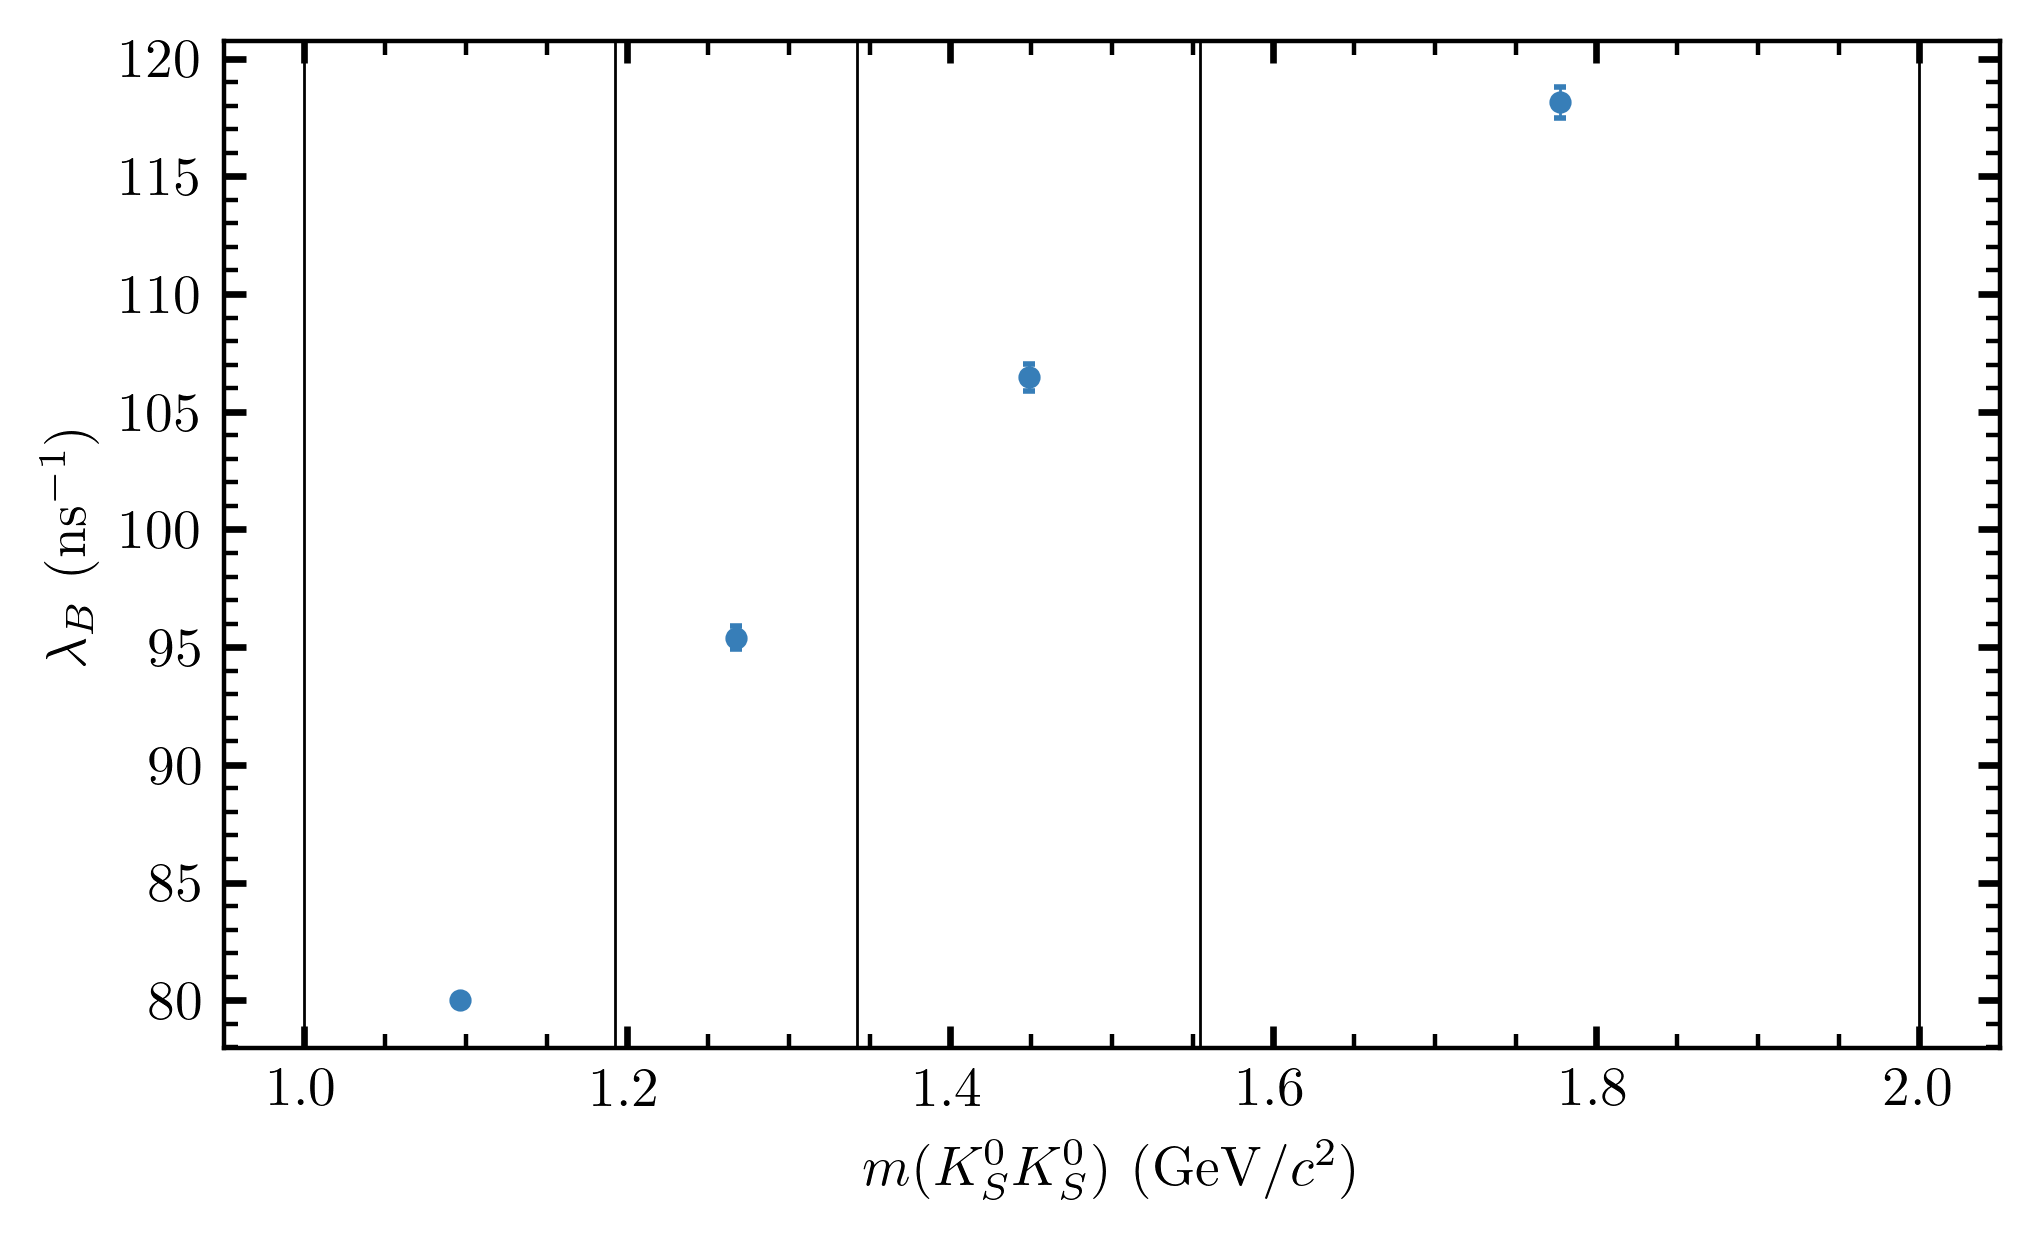
\includegraphics[width=0.8\textwidth]{figures/factorization_plot_data_chisqdof_3.4_4_quantiles.png}
  \end{center}
  \caption{Background exponential slopes from fits over four quantiles in $m(K_S^0K_S^0)$ ($x$-axis) of the rest-frame lifetime distributions of data. Both show a definite statistical dependence between rest-frame lifetime and the invariant mass of $K_S^0K_S^0$ with a p-value smaller than machine precision ($p < 2.23 \times 10^{-308}$).}\label{fig:factorization}
\end{figure}

\subsection{Application of Weights}\label{sec:application-of-weights}

The only thing left to do is determine how many background components we should use in the weighting procedure. To this end, we now turn to the Monte Carlo simulations of the $4\pi$-background. By choosing a number of quantiles in invariant mass corresponding to the number of components, we can fit single exponential distributions to each quantile in the simulated background. For instance, if we chose to use three background components, we would divide the background Monte Carlo into three, and fit each quantile to an exponential distribution to obtain a set of three $\lambda_B$ values. The resulting  $\lambda_B$ values could then be used as a starting point for a multi-component fit to the data. Alternatively, the background slopes could be fixed to the values from the fits to simulations, and only the yields would be allowed to float in the fit to data. We will refer to the first case, where the fit parameters ($\lambda_B$) from Monte Carlo are free, as $A$, the case where they are fixed as $B$ (the fit fraction $z$ is free in both cases). To select a model, we can use the relative Akaike Information Criterion (AIC)~\cite{Akaike1998} and the relative Bayesian Information Criterion (BIC)~\cite{Schwarz1978}:
\begin{alignat}{2}
  r\text{AIC} &\equiv \text{AIC} - \text{AIC}_\text{min} \quad\text{where } \text{AIC} &&\equiv 2k - 2\ln\mathcal{L} \\
  r\text{BIC} &\equiv \text{BIC} - \text{BIC}_\text{min} \quad\text{where } \text{BIC} &&\equiv k\ln{N} - 2\ln\mathcal{L},
  \label{eq:information-criteria}
\end{alignat}
where $k$ is the number of free parameters and $N$ is the number of events in the dataset. The optimal model will minimize these criteria. In \Cref{tab:splot-model-results}, all of the relative AIC and BIC values are shown. In this table, the methods are labeled $A$ and $B$ as described above followed by the number of background components in the fit. Since the procedure requires us to minimize $r\text{AIC}$ and $r\text{BIC}$, we can see that either method $A2$ or $A3$ should be the selected model. We can see the fit results in \Cref{fig:splot-A2-A3}. The fit for $A3$ contains two background components with very similar slopes, so we will prefer $A2$ for simplicity and will use it in the rest of the analysis. It is interesting to note that method $B$, where the component slopes were fixed to values obtained from fits over background Monte Carlo, are generally much poorer fits overall, despite having fewer degrees of freedom. This possibly reflects the fact that we only modeled one source of background in the Monte Carlo, while many sources could be present in the data.

\begin{table}
  \begin{center}
    \begin{tabular}{ccc}\toprule
      Method & $r\text{AIC}$ & $r\text{BIC}$\\\midrule
      $A1$ & $9544.558$ & $9515.780$\\
      $A2$ & $6.616$ & \underline{$0.000$}\\
      $A3$ & \underline{$0.000$} & $15.545$\\
       $A4$ & $9.318$ & $47.024$\\\midrule
      $B1$ & $9565.583$ & $9525.725$\\
       $B2$ & $9240.874$ & $9212.096$\\
       $B3$ & $9059.066$ & $9041.369$\\
       $B4$ & $9036.816$ & $9030.199$\\\bottomrule
    \end{tabular}
    \caption{Relative AIC and BIC values for each fitting method. The absolute minimum values in each column are underlined. Methods are labeled by whether the background slopes are free ($A$) or fixed ($B$) and by the number of background components used.}\label{tab:splot-model-results}
  \end{center}
\end{table}

\begin{figure}
  \begin{center}
    \begin{subfigure}[t]{\textwidth}
        \begin{center}
          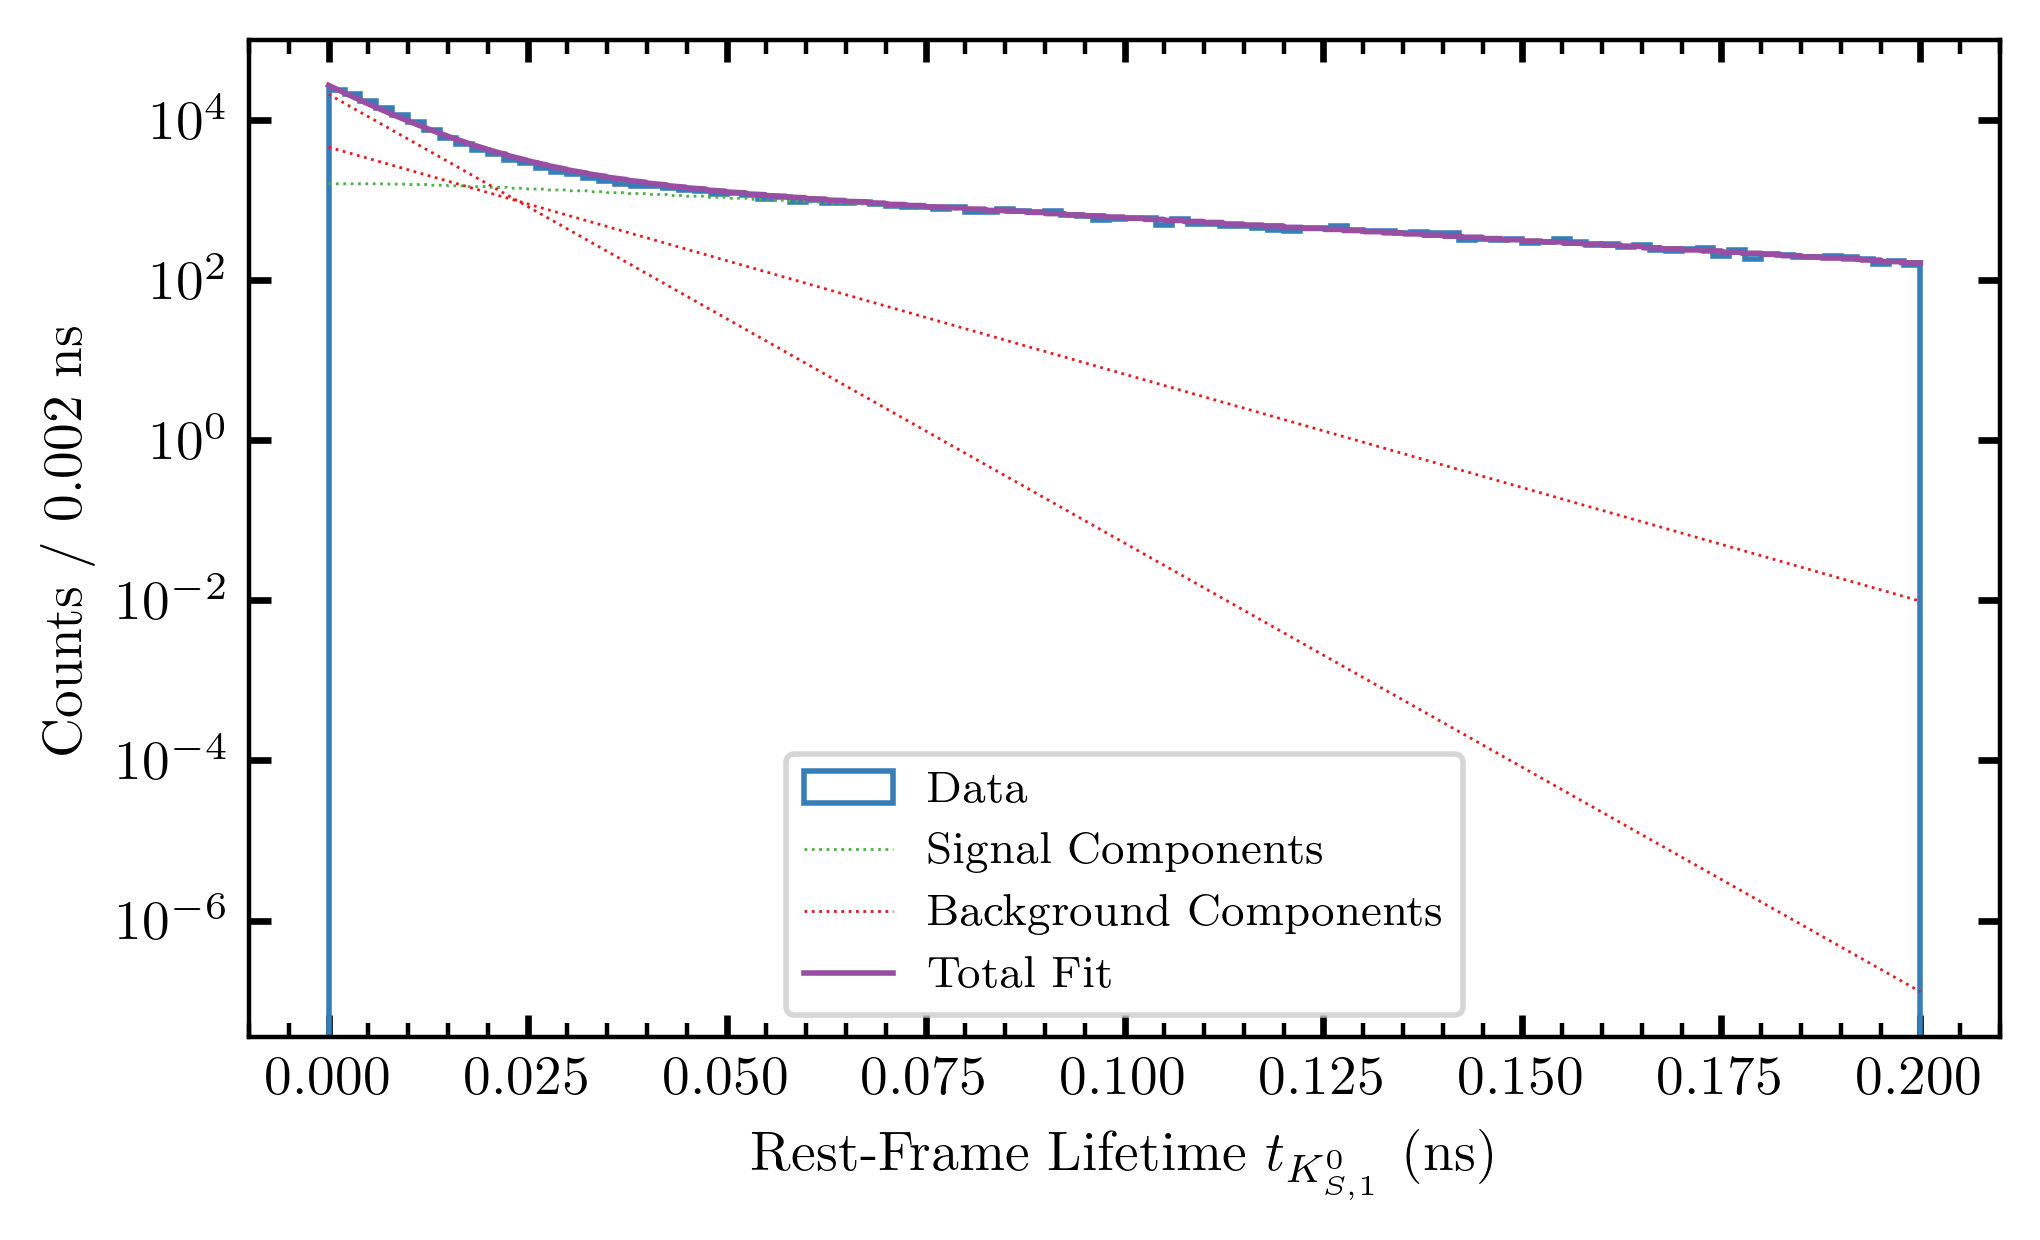
\includegraphics[width=.8\columnwidth]{figures/splot_fit_data_chisqdof_3.4_splot_D_1s_2b.png}
        \caption{The fit to data using method $A2$.}
        \end{center}
        \end{subfigure}
        \begin{subfigure}[t]{\textwidth}
          \begin{center}
            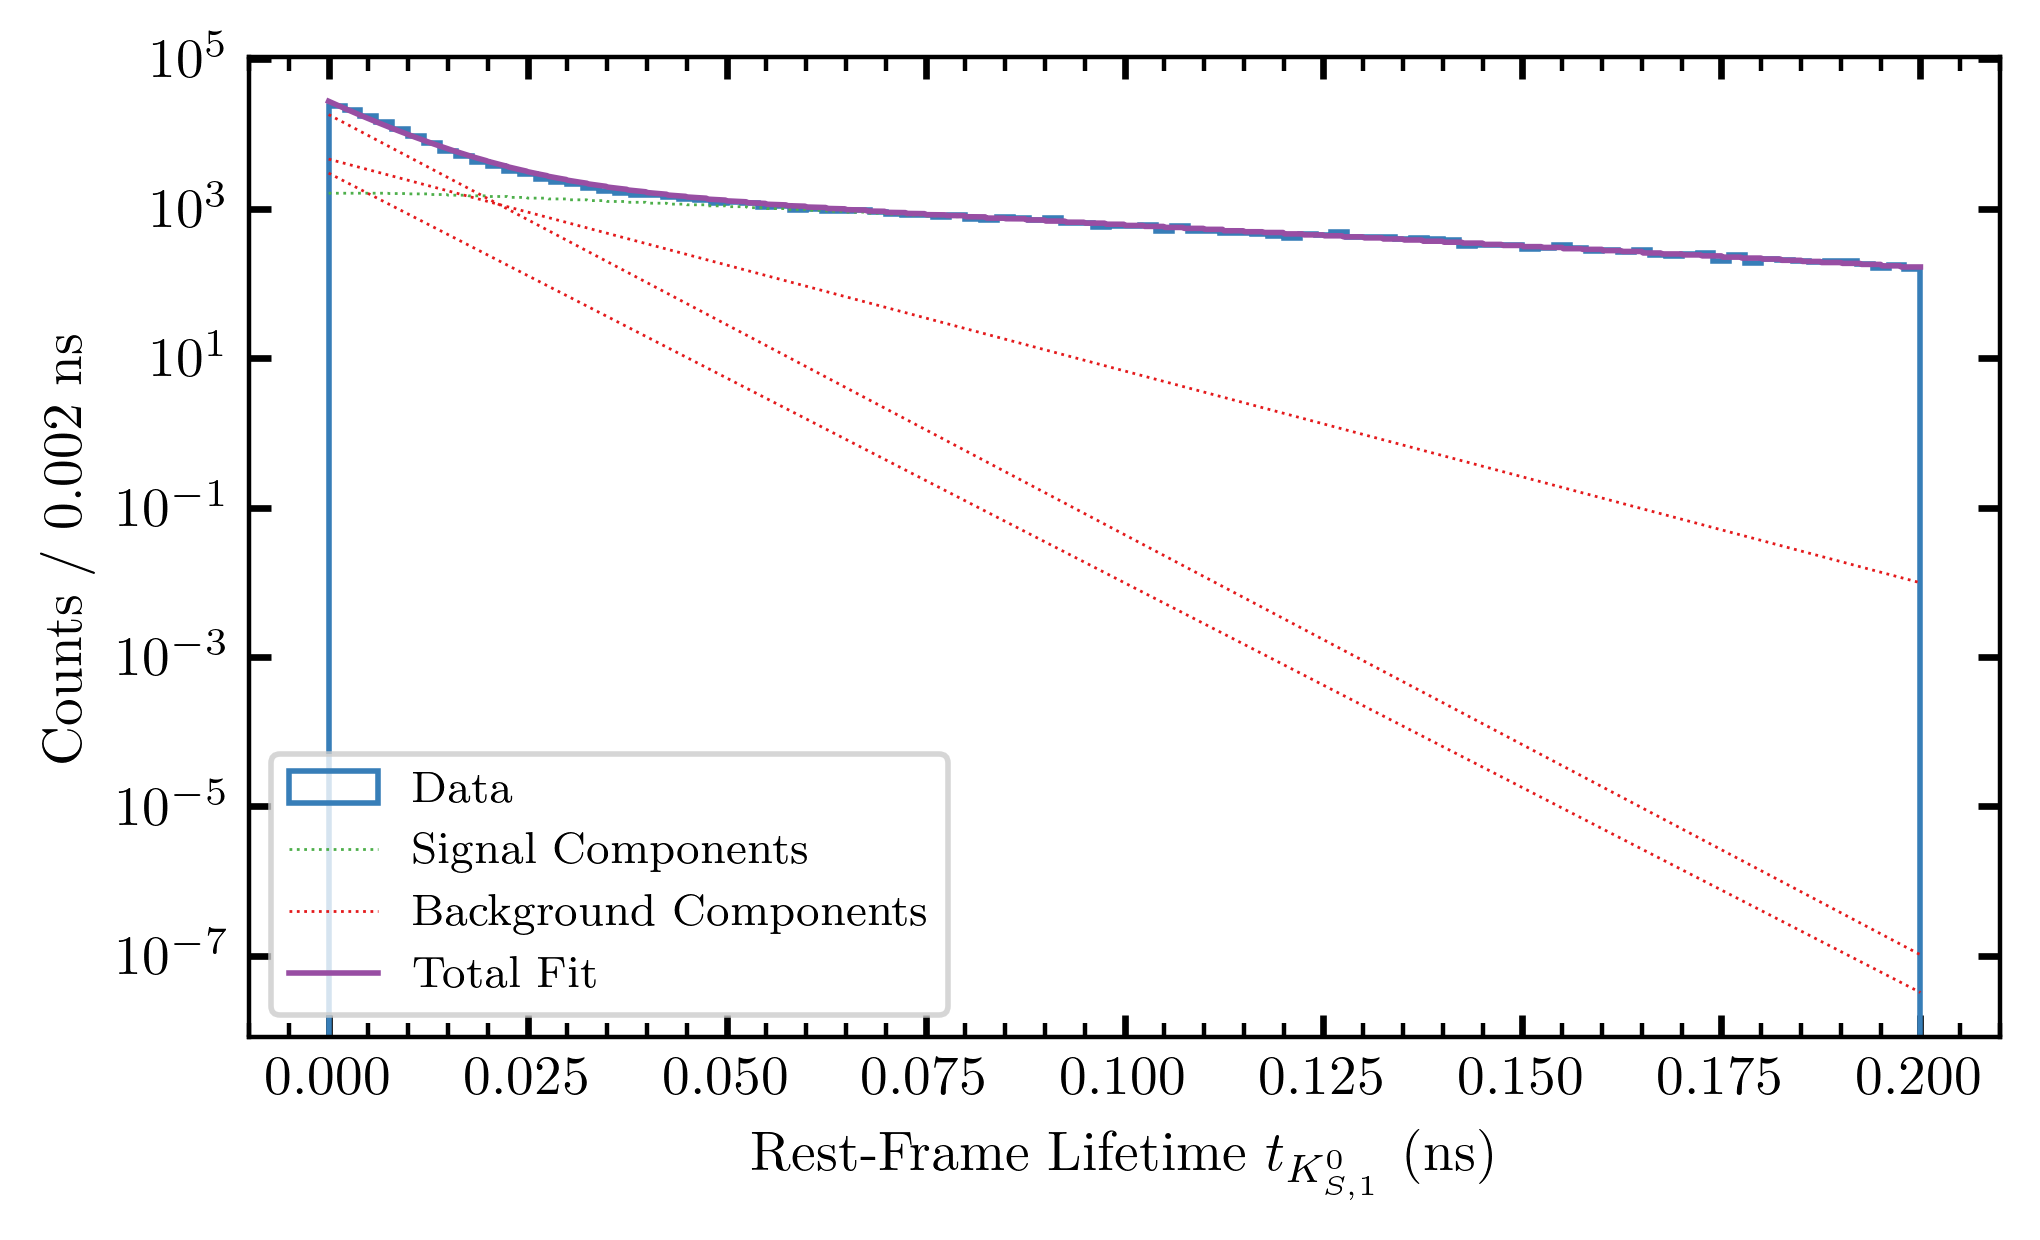
\includegraphics[width=.8\columnwidth]{figures/splot_fit_data_chisqdof_3.4_splot_D_1s_3b.png}
        \caption{The fit to data using method $A3$.}
          \end{center}
        \end{subfigure}
        \caption{Fits of \Cref{eq:splot-mixture} to data using method (a) $A2$ and (b) $A3$. The $A2$ configuration gives a better value for BIC, while $A3$ has a better AIC. We will use $A2$, since two of the background components of $A3$ are very similar and complicate the model unnecessarily.}\label{fig:splot-A2-A3}
\end{center}
\end{figure}

{\color{red}TODO: Plots of $E_\gamma$, invariant mass with/without baryon cut, baryon mass, $\cos\theta_{HX}$ and $\phi_{HX}$ vs invariant mass with and without baryon cut.}
